\lecture{4}{3. September 2025}{Control volume analysis II: Momentum \& energy equation}

\exercise{4.17}
Water is flowing steadily through the \ang{180} elbow shown. At the inlet to the elbow the gage pressure is \qty{103}{kPa}. The water discharges to atmospheric pressure. Assume properties are uniform over the inlet and outlet areas: $A_1 = \qty{2500}{mm^2}$, $A_2 = \qty{650}{mm^2}$, and $V_1 = \qty{3}{\frac{m}{s}}$. Find the horizontal component of force required to hold the elbow in place.


\begin{figure} [ht]
  \centering
  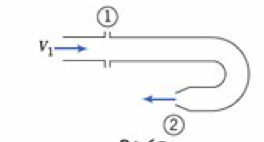
\includegraphics[width=0.25\linewidth]{./figures/e4_17.png}
\end{figure}

\bigbreak
The momentum equation in the $x$-direction is:
\[ 
R_x + F_{S_x} + F_{B_x} = \frac{\partial}{\partial t} \int_{\mathrm{CV}} u \rho \, \mathrm{d}V + \int_{\mathrm{CS}} u \rho \textbf{V} \cdot \mathrm{d}\textbf{A}
.\]
As we are seeking the horizontal force on the elbow we can neglect the gravitational force (i.e. $F_{B_x} = 0$). The pressure force is simply:
\[ 
F_{S_x} = p_1 A_1
.\]
As we assume steady flow we simply get:
\begin{align*}
R_{x} + p_1 A_1 &= V_1 \left( - \rho V_1 A_1 \right) - V_2 \left( \rho V_2 A_2 \right) \\
R_x &= - p_1 A_1 - \rho \left( V_1^2 A_1 + V_2^2 A_2 \right)
.\end{align*}
From the continuity equation we can calculate the outlet velocity $V_2$ as:
\begin{align*}
  0 &= - \rho V_1 A_1 + \rho V_2 A_2 \\
  V_2 &= \frac{V_1 A_1}{A_2} \\
  V_2 &= \qty{3}{\frac{m}{s}} \cdot \frac{\qty{2500}{mm}^2}{\qty{650}{mm}^2} \\
      &= \qty{11,54}{\frac{m}{s}}
.\end{align*}
Now all parameters in the equation for $R_x$ are known and it can be found as:
\begin{align*}
  R_x &= -\qty{103}{kPa} \cdot \qty{2500}{mm^2} - \qty{1000}{\frac{kg}{m^3}} \left( \left( \qty{3}{\frac{m}{s}}  \right)^2 \cdot \qty{2500}{mm^2} + \left( \qty{11,54}{\frac{m}{s}}  \right)^2 \cdot \qty{650}{mm^2} \right) \\
      &= - \qty{366,56}{N} 
.\end{align*}
Therefore a force of \qty{366,56}{N} directed against the wall is needed to hold the elbow in place. 


\exercise{4.16}
Water flows steadily through a fire hose and nozzle. The hose is \qty{35}{mm} in diameter and the nozzle tip is \qty{25}{mm} in diameter; water gage pressure in the hose is \qty{510}{kPa}, and the stream leaving the nozzle is uniform. The exit speed and pressure are \qty{32}{m/s} and atmospheric, respectively. Find the force transmitted by the coupling between the nozzle and hose. Indicate whether the coupling is in tension or compression. 

\begin{figure} [ht]
  \centering
  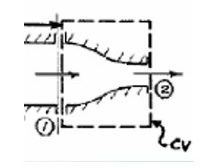
\includegraphics[width=0.25\linewidth]{./figures/e4_16.png}
\end{figure}
\bigbreak
Here the same formula as above (momentum in a control volume) can be used as:
\[ 
R_x + F_{S_x} + F_{B_x} = \frac{\partial }{\partial t} \int_{\mathrm{CV}} u \rho \, \mathrm{d}V + \int_{\mathrm{CS}} u \rho \textbf{V} \cdot \mathrm{d}\textbf{A}
.\]
With the same assumption of steady flow as above we get:
\[ 
R_x + p_1 A_1 = V_2 \left( \rho V_2 A_2 \right) - V_1 \left( \rho V_1 A_1 \right)
.\]
For incompressible steady flow we have:
\[ 
  0 = - \rho_1 V_1 A_1 + \rho_2 V_2 A_2 \implies V_1 = V_2 \frac{A_2}{A_1} = V_2 \left( \frac{D_2}{D_1} \right)^2 = \qty{32}{\frac{m}{s}} \cdot \left( \frac{\qty{25}{mm} }{\qty{35}{mm} } \right)^2 = \qty{16,33}{\frac{m}{s}} 
.\]
The condition from above can also be used to rewrite the expression from before as:
\begin{align*}
  R_x + p_1 A_1 &= V_2 \left( \rho V_2 A_2 \right) - V_1 \left( \rho V_1 A_1 \right) \\
  R_x &= V_2 \left( \rho V_2 A_2 \right) - V_1 \left( \rho V_1 A_1 \right) - p_1 A_1 \\
  &= V_2 \left( \rho V_2 A_2 \right) - V_1 \left( \rho V_2 A_2 \right) - p_1 A_1 \\
  &= \left( \rho V_2 A_2 \right) \left( V_2 - V_1 \right) - p_1 A_1
.\end{align*}
Plugging in all the known values we get:
\[ 
R_x = \left( \qty{1000}{\frac{kg}{m^3}} \cdot \qty{32}{\frac{m}{s}} \cdot \pi \cdot \left( \qty{12,5}{mm}  \right)^2 \right) \left( \qty{32}{\frac{m}{s}} - \qty{16,33}{\frac{m}{s}}  \right) - \qty{510}{kPa} \cdot \pi \cdot \left( \qty{17,5}{mm}  \right)^2 = - \qty{245}{N}
.\]
Therefore a force of $R_x = - \qty{245}{N}$ would be applied to the nozzle. The sign tells us that the force acts against the control volume to the left meaning the nozzle must itself be in tension.


\exercise{4.14}
The radial-flow turbine in an automotive turbocharger has a diameter of \qty{60}{mm} and rotates at \qty{100000}{RPM}. An air flow of \qty{0,016}{kg/s} enters the turbine wheel at \qty{60}{m/s} and an angle of \ang{25} as shown in \autoref{fig:e4_14}. The air flow leaving has negligible angular momentum. Determine the power (\unit{W} and \unit{hp}) the turbine produces.

\begin{figure} [ht]
  \centering
  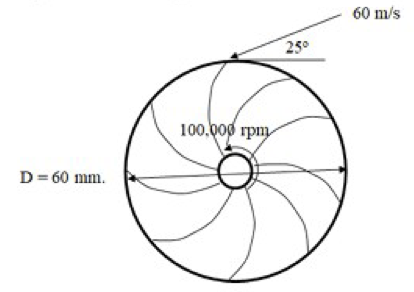
\includegraphics[width=0.25\linewidth]{./figures/e4_14.png}
  \caption{}
  \label{fig:e4_14}
\end{figure}

\bigbreak
In this exercise the angular-momentum principle for an inertial reference system will be used. It is:
\[ 
\textbf{r} \times \textbf{F}_s + \int_{\mathrm{CV}} \textbf{r} \times \textbf{g} \rho \, \mathrm{d}V + \textbf{T}_{\mathrm{shaft}} = \frac{\partial }{\partial t} \int_{\mathrm{CV}} \textbf{r} \times \textbf{V} \rho \, \mathrm{d}V + \int_{\mathrm{CS}} \textbf{r} \times \textbf{V} \rho \textbf{V} \cdot \mathrm{d}\textbf{A}
.\]
As we assume that there is no body or surface forces acting on the system and that the flow is steady this reduces to:
\[ 
\textbf{T}_{\mathrm{shaft}} = \int_{\mathrm{CS}} \textbf{r} \times \textbf{V} \rho \textbf{V} \cdot \mathrm{d}\textbf{A}
.\]
In scalar form this becomes
\[ 
T_{\mathrm{shaft}} = r_o V_{\mathrm{tan}} \rho Q = r_0 V_{\mathrm{tan}} \dot{m}
.\]
The tangential velocity is the component of the velocity tangent to the impeller as
\[ 
V_{\mathrm{tan}} = \qty{60}{\frac{m}{s}} \cdot \cos \ang{25} = \qty{54,4}{\frac{m}{s}} 
.\]
And therefore the torque produced by the rotor is:
\[ 
T_{\mathrm{shaft}} = r_o V_{\mathrm{tan}} \dot{m} = \frac{\qty{60}{mm}}{2} \cdot \qty{54,4}{\frac{m}{s}} \cdot  \qty{0,016}{\frac{kg}{s}} = \qty{0,0261}{N.m} 
.\]
The power produced is given as:
\[ 
\dot{W} = T_{\mathrm{shaft}} \omega
\]
where $\omega$ is the rotational frequency. The speed of \qty{1600}{RPM} is therefore converted to frequency as:
\[ 
\omega = \qty{100000}{RPM} \cdot 2\pi \unit{rev^{-1}} \cdot \frac{\unit{min}}{\qty{60}{s}} = \qty{10470}{s^{-1}} 
.\]
Therefore the power is:
\[ 
\dot{W} = T_{\mathrm{shaft}} \cdot \omega = \qty{0,0261}{N.m} \cdot \qty{10470}{s^{-1}} = \qty{273}{W} = \qty{0,367}{hp} 
.\]

